%\author{traduit par Jérémy Garniaux}

% vim: set textwidth=78 autoindent:

\section{Les extensions de QGIS}\label{sec:extensions}\index{extensions}

% when the revision of a section has been finalized, 
% comment out the following line:
%\updatedisclaimer

%QGIS has been designed with a plugin architecture.
%This allows new features/functions to be easily added to the application.
%Many of the features in QGIS are actually implemented as \textbf{core} or \textbf{external} plugins.\index{plugins!types} 

QGIS repose sur un système d'extensions.
Ce dernier permet d'ajouter facilement de nouvelles fonctions au logiciel. 
De nombreuses nouvelles fonctions de QGIS sont implémentées comme des extensions \textbf{principales} ou \textbf{complémentaires}. \index{plugins!types} 

%\begin{itemize}
%\item \textbf{Core Plugins} are maintained by the QGIS Development Team and are automatically part of every QGIS distribution.
%They are written in one of two languages: C++ or Python.
%More information about core plugins are provided in Section \ref{sec:core_plugins}.
%\item \textbf{External Plugins} are currently all written in Python.
%They are stored in external repositories and maintained by the individual author.
%They can be added to QGIS using the core plugin called \filename{Plugin Installer}.
%More information about external plugins are provided in Section \ref{sec:external_plugins}.
%\end{itemize}

\begin{itemize}
\item Les \textbf{extensions principales} sont maintenues par l'équipe de développement de QGIS et sont intégrées automatiquement à chaque nouvelle distribution de QGIS.
Elles sont écrites en C++ ou en Python.
On trouvera plus d'informations sur les extensions principales dans la Section \ref{sec:core_plugins}.
\item Les \textbf{extensions complémentaires} sont actuellement toutes écrites en Python.
Elles sont stockées dans des dépôts externes et maintenues par leurs auteurs.
Elles peuvent être ajoutées à QGIS en utilisant l'extension principale nommée \filename{Gestionnaire d'extensions}.
On trouvera plus d'informations sur les extensions complémentaires dans la Section \ref{sec:external_plugins}.
\end{itemize}

%\subsection{Managing Plugins}\label{sec:managing_plugins}
%\index{plugins!managing} 
%
%Managing plugins in general means loading or unloading them using the \filename{Plugin Manager} plugin.
%External plugins need to be first installed using the \filename{Plugin Installer} plugin.

\subsection{Gérer les extensions}\label{sec:managing_plugins}
\index{plugins!managing} 

De manière générale, gérer les extensions consiste à les afficher ou pas à l'aide du \filename{Gestionnaire d'extension}.
Les extensions complémentaires doivent d'abord être installées à l'aide du \filename{Gestionnaire d'extension}.

%\subsubsection{Loading a QGIS Core Plugin}\label{sec:load_core_plugin} 

%Loading a QGIS Core Plugin is provided in the main menu \mainmenuopt{Plugins} > \dropmenuopttwo{mActionShowPluginManager}{Manage Plugins...}.\index{plugins!manager}

%\begin{figure}[ht]
%   \begin{center}
%   \caption{Plugin Manager \nixcaption}\label{fig:pluginmanager}\smallskip
%   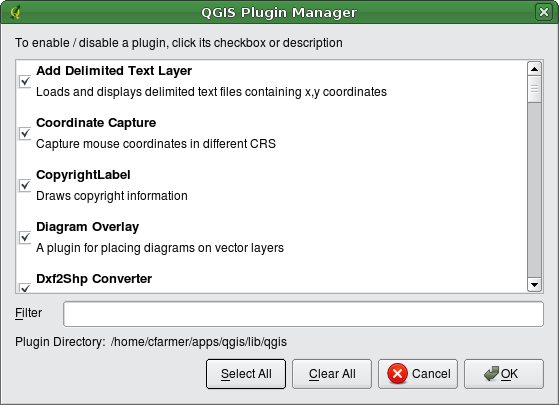
\includegraphics[clip=true, width=14cm]{pluginmanager}
%\end{center}
%\end{figure}

%The Plugin Manager lists all the available plugins and their status (loaded or unloaded).
%All available means all core plugins and all external plugins you added using \filename{Plugin Installer} plugin (see Section \ref{sec:external_plugins}). 
%Figure \ref{fig:pluginmanager} shows the Plugin Manager dialog.
%Loaded plugins are "remembered" when you exit the application and restored the next time you run QGIS.

%\begin{Tip}\caption{\textsc{Crashing Plugins}}\index{crashes}
%\qgistip{If you find that QGIS crashes on startup, a plugin may be at fault.
%You can stop all plugins from loading by editing your stored settings file (see \ref{subsec:gui_options} for location).
%Locate the plugins settings and change all the plugin values to false to prevent them from loading.
%\nix {For example, to prevent the Delimited text plugin from loading, the entry in \$HOME/.config/QuantumGIS/qgis.conf on Linux should look like this:\usertext{Add %Delimited Text Layer=false}.}
%\normalfont 
%Do this for each plugin in the [Plugins] section.
%You can then start QGIS and add the plugins one at a time from the Plugin Manger to determine which is causing the problem.}
%\end{Tip} 

\subsubsection{Installer une extension principale}\label{sec:load_core_plugin} 

On installe une extension principale à l'aide du menu \mainmenuopt{Plugins} > \dropmenuopttwo{mActionShowPluginManager}{Gestionnaire d'extension...}.\index{plugins!manager}

\begin{figure}[ht]
   \begin{center}
   \caption{Gestionnaire d'extension \nixcaption}\label{fig:pluginmanager}\smallskip
   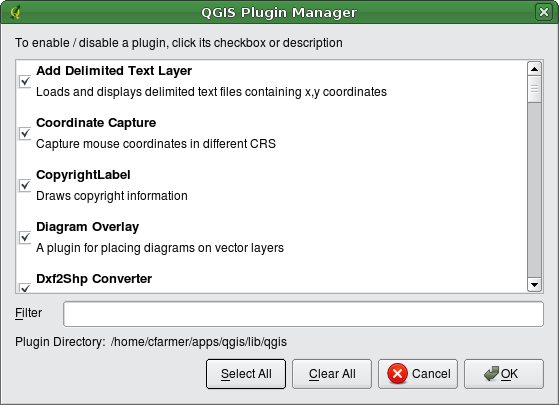
\includegraphics[clip=true, width=14cm]{pluginmanager.png}
\end{center}
\end{figure}

Le gestionnaire d'extension liste toutes les extensions disponibles et leur statut (installé ou pas).
"Tous disponibles" signifie que toutes les extensions principales ou complémentaires que vous avez ajoutées à l'aide de l'extension \filename{Gestionnaire d'Extension} (see Section \ref{sec:external_plugins}). 
La figure \ref{fig:pluginmanager} montre la boîte de dialogue du Gestionnaire d'extension.
Les extensions installées sont mémorisées lorsque vous quittez l'application et seront restaurées à la prochaine ouverture de QGIS.

\begin{Astuce}\caption{\textsc{Extensions et plantages}}\index{crashes}
\qgistip{Si votre installation de QGIS plante au démarrage, une extension est peut-être en cause.
Vous pouvez éviter le chargement des extensions en éditant votre fichier de configuration (voir \ref{subsec:gui_options} pour localiser ce fichier).
Localisez la configuration de l'extension et changez toutes les valeurs à "false" pour empêcher leur chargement.
\nix Par exemple, pour éviter le chargement de l'extension "Ajouter une couche texte délimitée", l'entrée de \$HOME/.config/QuantumGIS/qgis.conf doit ressembler à \usertext{Add Delimited Text Layer=false}.
\normalfont 
Faites de même pour chaque extension dans la section [Extension].
Vous pouvez ensuite démarrer QGIS et ajouter les extensions une à la fois depuis le Gestionnaire d'extension pour déterminer celle qui est la source du problème.}
\end{Astuce}

%\subsubsection{Loading an external QGIS Plugin}\label{sec:load_external_plugin} 

%To be able to integrate external plugins into QGIS you first need to load the \filename{Plugin Installer} plugin as desribed in Section \ref{sec:load_core_plugin}.
%Then you can load external QGIS python plugin in two steps: 

%\begin{enumerate}
%\item Download an external plugin from a repository using the \filename{Plugin Installer} (Section \ref{sec:python_plugin_installer}).
%The new external plugin will be integrated into the list of available plugins in the \filename{Plugin Manager}.
%\item Load the plugin using the \filename{Plugin Manager}.
%\end{enumerate}

\subsubsection{Installer une extension complémentaire de QGIS}\label{sec:load_external_plugin} 

Afin de pouvoir intégrer des extensions complémentaires dans QGIS, vous devez d'abord installer l'extension \filename{Gestionnaire d'extension} comme décrit dans la Section \ref{sec:load_external_plugin}.
Les extensions python complémentaires peuvent ensuite être installées en deux étapes :

\begin{enumerate}
\item Télechargez une extension complémentaire depuis un dépôt à l'aide de l'\filename{Installeur d'extension python} (Section \ref{sec:python_plugin_installer}).
La nouvelle extension complémentaire sera intégrée dans la liste des extensions disponibles du \filename{Gestionnaire d'extension}.
\item Installez l'extension à l'aide du \filename{Gestionnaire d'extension}.
\end{enumerate}

%\subsubsection{Using the QGIS Python Plugin Installer}\index{plugins!installing}\label{sec:python_plugin_installer}
%\index{plugins!Python Plugin Installer}\index{plugins!upgrading}

%\begin{figure}[ht]
%   \begin{center}
%   \caption{Installing external python plugins \nixcaption}
%\label{fig:plugininstaller}\smallskip
%   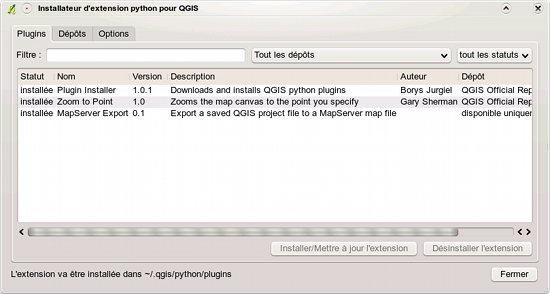
\includegraphics[clip=true, width=14cm]{plugininstaller}
%\end{center}
%\end{figure}

\subsubsection{Utiliser l'installeur d'extension python de QGIS}\index{plugins!installing}\label{sec:python_plugin_installer}
\index{plugins!Python Plugin Installer}\index{plugins!upgrading}

\begin{figure}[ht]
   \begin{center}
   \caption{Installer des extensions complémentaires python\nixcaption}
\label{fig:plugininstaller}\smallskip
   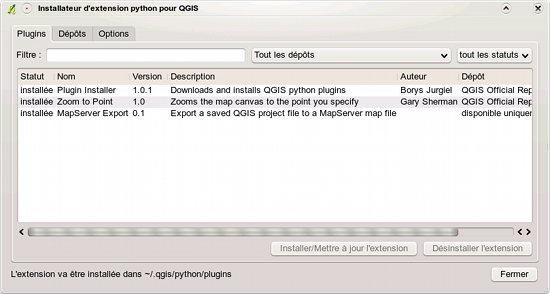
\includegraphics[clip=true, width=14cm]{plugininstaller}
\end{center}
\end{figure}

%In order to download and install an external Python plugin, click the menu \mainmenuopt{Plugins} > \dropmenuopttwo{plugin_installer}{Fetch Python Plugins...}.
%The \filename{Plugin Installer} window will appear (figure \ref{fig:plugininstaller}) with the tab \tab{Plugins}, containing the list of all Python plugins available in remote repositories as well as installed ones. Each plugin can be either:
%\begin{itemize}
%\item \textbf{not installed} - it means the plugin is available in the repository, but is not installed yet. In order to install, select it from the list and click the \button{Install plugin} button.
%\item \textbf{new} - the same as before but the plugin is seen for the first time.
%\item \textbf{installed} - the plugin is installed. If it's also available in any repository the \button{Reinstall plugin} button is enabled. But if the available version is older than the installed one, the \button{Downgrade plugin} button appears instead.
%\item \textbf{upgradeable} - the plugin is installed, but there is an updated version available. The \button{Upgrade plugin} button is enabled.
%\item \textbf{invalid} - the plugin is installed, but is unworkable. The reason is explained in the plugin description.
%\end{itemize}

Pour télécharger et installer une extension python complémentaire, cliquez  sur le menu \mainmenuopt{Plugins} > \dropmenuopttwo{plugin_installer.png}{Récupération des extensions python...}.
La fenêtre de l'\filename{Installeur d'extension python} apparaîtra (figure \ref{fig:plugininstaller}) avec l'onglet \tab{Plugins}, qui présente la liste de toutes les extensions python installées ou disponibles dans des dépôts distants. Chaque extension peut-être soit :
\begin{itemize}
\item \textbf{non installée} - signifie que l'extension est disponible dans le dépôt, mais n'est pas encore installée. Pour l'installer, sélectionnez-la dans la liste et cliquez sur le bouton \button{Installer l'extension}.
\item \textbf{nouveau} - même statut que ci-dessus, mais l'extension apparaît pour la première fois.
\item \textbf{installée} - l'extension est installée. Si elle est également disponible dans un dépôt, le bouton \button{Ré-installer l'extension} est actif. En revanche, si la version disponible est plus ancienne que la version installée, le bouton \button{???} apparaît à la place.
\item \textbf{mise à jour} - l'extension est installée, mais une version plus récente est disponible, le bouton \button{Mise à jour de l'extension} est actif.
\item \textbf{invalide} - l'extension est installée, mais ne fonctionne pas. Les détails sont donnés dans la description de l'extension.
\end{itemize}

%\minisec{Plugins tab}
%
%To install a plugin, select it from the list and click the \button{Install plugin} button. The plugin is installed in its own directory, e.g. for \nix under \filename{\$HOME/.qgis/python/plugins} and is only visible for the user who has installed it. See a list of other OS specific subdirectory used for plugins in Section~\ref{subsec:pyfoursteps}. If the installation is successful, a confirmation message will appear. Then you need go to the \mainmenuopt{Plugins} > \dropmenuopttwo{mActionShowPluginManager}{Manage Plugins...} and load the installed plugin. 
%
%If the installation fails, the reason is displayed. The most often troubles are related to connection errors and missing Python modules. In the former case you'll probably need to wait some minutes or hours, in the latter one you need to install the missing modules in your operating system prior to using the plugin. \nix{For Linux, most required modules should be available in a package manager}. \win{For install instructions in Windows visit the module home page}. If you use a proxy, you may need to configure it under the menu \mainmenuopt{Settings} > \dropmenuopttwo{mActionOptions}{Options} on the \tab{Proxy} tab.
%
%The \button{Uninstall plugin} button is enabled only if the selected plugin is installed and it's not a core plugin. Note that if you have installed an update of a core plugin, you can still uninstall this update with the \button{Uninstall plugin} and revert to the version shipped within Quantum GIS install package. This one cannot be uninstalled.

\minisec{Onglet Plugins}

Pour installer une extension, sélectionnez-la dans la liste et cliquez sur le bouton \button{Installer l'extension}. L'extension est installée dans son propre répertoire, par ex. pour \nix dans \filename{\$HOME/.qgis/python/plugins} et n'est visible que pour l'utilisateur qui l'a installée. Voir une liste des répertoires d'installation des extensions sous d'autres OS dans la Section~\ref{subsec:pyfoursteps}. Si l'installation réussit, un message de confirmation apparaît. Cliquez ensuite sur le menu \mainmenuopt{Plugins} > \dropmenuopttwo{mActionShowPluginManager}{Gestionnaire d'extension...} et chargez l'extension fraîchement installée.
and load the installed plugin.

Si l'installation ne fonctionne pas, la raison est indiquée. Les problèmes les plus fréquents sont dus à des erreurs de connexion et à des modules Python manquants. Dans le premier cas, il vous faudra probablement attendre quelques minutes ou heures ; dans le second cas, il sera nécessaire d'installer les modules manquants avant d'utiliser les extensions. \nix{Pour Linux, les modules les plus recherchés devraient être disponibles dans un gestionnaire de paquets}. \win{Pour des installations d'instruction dans Windows, visitez la page web du module}. Si vous utilisez un proxy, vous pourrez avoir besoin de le configurer dans le menu \mainmenuopt{Préférences} > \dropmenuopttwo{mActionOptions}{Options} dans l'onglet \tab{Proxy}.

Le bouton \button{Désinstaller l'extension} est actif seulement si l'extension sélectionnée est installée et n'est pas une extension principale. Notez que si vous avez installé une mise à jour d'une extension principale, il est toujours possible de désinstaller cette mise à jour avec le bouton \button{Désinstaller l'extension} et revenir à la version d'origine fournie à l'installation de Quantum GIS. Cette dernière ne peut pas être désinstallée.

%\minisec{Repositories tab}
%
%The second tab \tab{Repositories} contains a list of plugin repositories available for the Plugin Installer. By default, only the QGIS Official Repository is used. You can add some user-contributed repositories, including the central QGIS Contributed Repository and a few author repositories by clicking the \button{Add 3rd party repositories} button. Those repositories contain a huge number of more or less useful plugins but please note that they aren't maintained by the QGIS Development Team and we can't take any responsibility for them. You can also manage the repository list manually, that is add, remove and edit the entries. Temporary disabling a particular repository is possible clicking the \button{Edit...} button.
%
%The \checkbox{Check for updates on startup} checkbox makes QGIS looking for plugin updates and news. If it's enabled, all repositories listed and enabled on the \tab{Repositories} tab are checked whenever the program is starting. If a new plugin or an update for one of installed plugins is available, a clickable notification appears in the Status Bar. If the checkbox is disabled, looking for updates and news is performed only when Plugin Installer is being launched from the menu.
%
%In case of some internet connection problems a \textit{Looking for new plugins...} indicator in the Status Bar may stay visible during whole QGIS session and cause a program crash when exiting. In this case please disable the checkbox.

\minisec{Onglet Dépôts}

Le second onglet \tab{Dépôts} contient une liste de dépôts d'extensions disponibles. Par défaut, seul le dépôt officiel de QGIS (QGIS Official Repository) est utilisé. Vous pouvez ajouter des dépôts contenant des contributions d'utilisateurs, notamment le dépôt de contributions de QGIS (QGIS Contributed Repository) et quelques dépôts d'auteurs en cliquant sur le bouton \button{Ajouter un dépôt-tiers d'extension à la liste}. Ces dépôts contiennent une grande quantité d'extensions plus ou moins utiles, mais veuillez noter qu'elles ne sont pas maintenues par l'équipe de développement de QGIS et que nous ne pouvons prendre aucune responsabilité pour elles. Vous pouvez également gérer la liste de dépôts manuellement, pour ajouter, retirer ou éditer des entrées. Désactiver temporairement un dépôt particulier est possible en cliquant sur le bouton \button{Editer}.


La case \checkbox{Chercher des mises à jour au démarrage} configure QGIS pour rechercher des mises à jour et des actualités relatives aux extensions. Si la case est cochée, tous les dépôts listés et activés dans l'onglet \tab{Dépôts} sont vérifiés à chaque démarrage du programme. Si une nouvelle extension ou une mise à jour pour une des extensions installées est disponible, une notification cliquable apparaît dans la barre de statut. Si la case est décochée, la recherche de mises à jour et d'actualités s'effectue uniquement lorsque l'Installeur d'Extension est lancé manuellement depuis le menu.

En cas de problèmes de connexion Internet, un indicateur \textit{Recherche de nouvelles extensions...} dans la barre de statut peut rester visible durant toute la session QGIS et faire planter le programme à la fermeture. Dans ce cas, décochez la case.

%\subsection{Data Providers}\index{data providers}
%
%Data Providers are "special" plugins that provides access to a data store.
%By default, QGIS supports PostGIS layers and disk-based data stores supported by the GDAL/OGR library (Appendix \ref{appdx_ogr}).
%A Data Provider plugin extends the ability of QGIS to use other data sources.
%
%Data Provider plugins are registered automatically by QGIS at startup.
%They are not managed by the Plugin Manager but used behind the scenes when a data type is added as a layer in QGIS.

\subsection{Fournisseurs de données}\index{data providers}

Les Fournisseurs de données sont des extensions "spéciales" donnant accès à un dépôt de données.
Par défaut, QGIS supporte les couches PostGIS et les bases de données fichiers couverts par la bibliothèque GDAL/OGR(Appendix \ref{appdx_ogr}).
L'utilisation d'extensions pour fournir des données permet d'élargir les sources de données utilisables par QGIS.

Les extensions fournissant des données sont automatiquement enregistrées par QGIS au démarrage.
Elles ne sont pas gérées par le Gestionnaire d'Extension, mais utilisées en arrière-plan lorsqu'un type de données est ajouté comme couche dans QGIS.
